% ********** Introduction **********
\chapter{Introduction}
\label{cha:introduction}

\epigraph{`Begin at the beginning,' the King said gravely, `and go on till you come to the end: then stop.'}{{\epiauthor Lewis Carroll}, Alice in Wonderland}

From astronomy to security and screening, there is a need for extremely fast highly-sensitive detectors operating in the mid to far infrared. In this work, one such detector---the silicon cold-electron bolometer---is introduced, tested and appraised.

\section{Motivation}\label{sec:motivation}
\subsection{Astronomy}
Millimetre and sub-millimetre wavelengths are of particular interest to several fields of astronomy, such as: studying the Cosmic Microwave Background (CMB), galactic astrophysics (including the study of cold dust), star formation, and cosmology\reminder{improve this}. This is due to the emission black-body radiation from cold sources at these frequencies (for example the cosmic microwave background has an average temperature of $2.73~\mathrm{K}$, with a spectrum peaking at $150~\mathrm{GHz}$). While the recent \textit{Herschel} and \textit{Planck} missions have provided a plethora of data in these fields recently, such missions are incredibly expensive; for example the cost of the entire four year \textit{Herschel} mission was $\euro{} 1.1~\mathrm{billion}$ \parencite[$\approx \$ 1.2~\mathrm{billion}$;][]{HerschelFactSheet}. This is comparable to the $\$ 1.4~\mathrm{billion}$ spent to develop the sixty six telescope Atacama Large Millimeter Array (ALMA) in Chile \parencite{ESO2013}, which, due to being ground based, has the potential to run indefinitely and is upgradeable.
\begin{figure}[tb]
\begin{center}
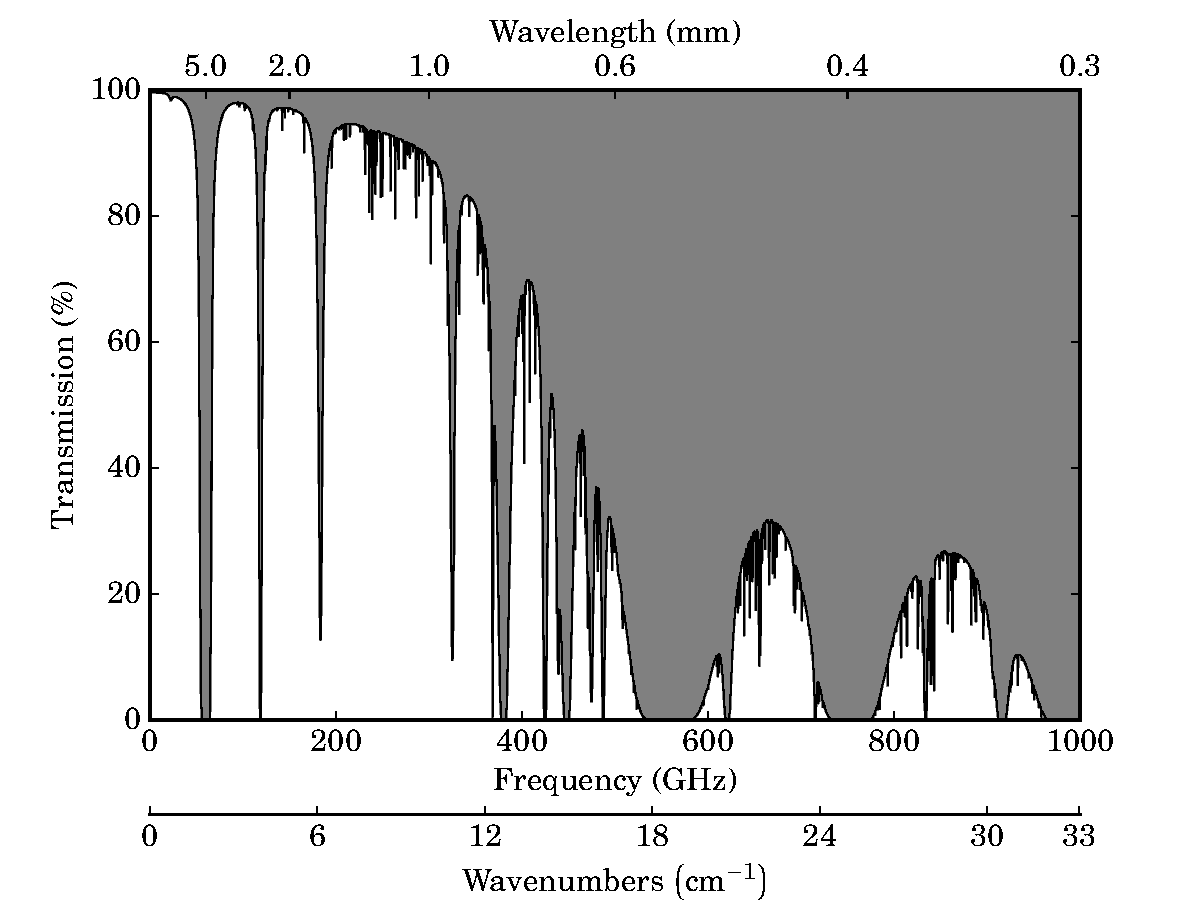
\includegraphics[width = 0.95\textwidth]{figures/MaunaKeaTransmission}
\caption[Atmospheric transmission at the summit of Mauna Kea in Hawaii]{Atmospheric transmission at the summit ($4,200~\mathrm{m}$ above sea level) of Mauna Kea in Hawaii. Calculated using the model presented by \textcite{Pardo2001}, assuming $1~\mathrm{mm}$ precipitable water vapour.}
\label{fig:MaunaKeaTransmission}
\end{center}
\end{figure}
\par
The ability to carry out astronomy at ground-based facilities is restricted by two main factors. Firstly, the black-body emission from the optical components of the telescope result in a high foreground power (i.e. brighter than the source). Secondly, the atmospheric transmission in the mid- to far-infrared is not perfect, in fact, for several frequency bands, the atmospheric transmission is essentially zero. Figure~\ref{fig:MaunaKeaTransmission} shows the transmission of light with frequencies below $1~\mathrm{THz}$ at the summit of the Mauna Kea Mountain in Hawaii, the site of the James Clerk Maxwell Telescope (JCMT), regarded to be one of the best sites in the world for observations at these frequencies. This figure assumes $1~\mathrm{mm}$ of perceptible water vapour in the atmosphere; this is equivalent to approximately the best $25~\%$ of all nights. 
\par 
This attenuation of radiation by the Earth's atmosphere is a key reason for launching space-based observatories. Such observatories are not only immune to the issues of attenuation from the atmosphere but also need not contest with the high backgrounds, which ground-based telescopes are subjected to. This allows space-based telescopes to study faint sources that are inaccessible to ground-based telescopes. 
\par 
An example of science which can be performed with both ground- and space-based instruments is the measurement of the cosmic microwave background. Some key frequencies used to observe this phenomenon are $70$, $150$, $220$, and $350~\mathrm{GHz}$; these frequencies are given by the specifications for the low- and high-frequency instruments on the \textit{Planck} satellite \parencite{Valenziano2007,Lamarre2003}. Figure~\ref{fig:MaunaKeaTransmission} shows that these frequencies are not heavily attenuated by the atmosphere and thus, can be observed from the ground as well as from space. An example of this work is the all-sky survey performed by \textit{Planck}, shown in Figure~\ref{fig:Planck_CMB}. Similar work has been performed by the ground-based Keck and BICEP arrays.
\begin{figure}[tb]
\begin{center}
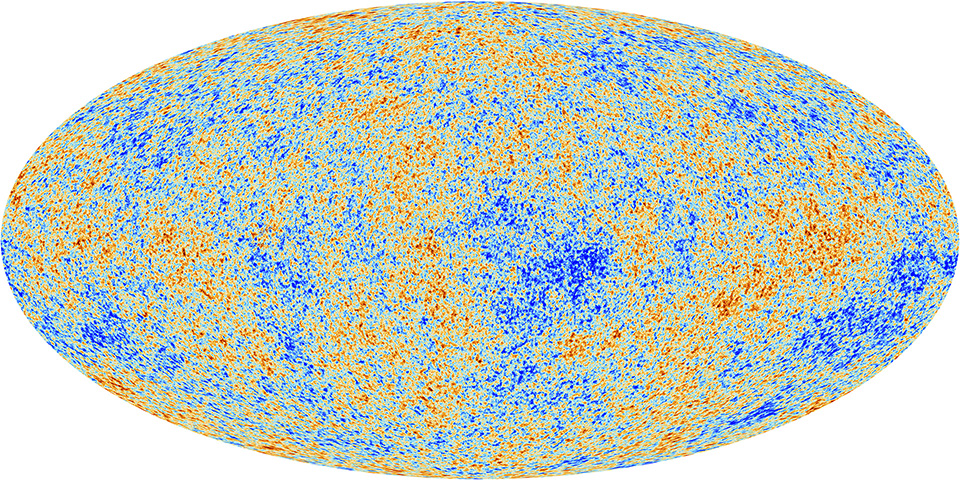
\includegraphics[width = 0.95\textwidth]{figures/Planck_CMB}
\caption[All-sky map of the cosmic microwave background produced by the \textit{Planck} mission]{All-sky map of the cosmic microwave background produced by the \textit{Planck} mission. \copyright~\gls{acr:ESA} and the \textit{Planck} Collaboration.}
\label{fig:Planck_CMB}
\end{center}
\end{figure}
\par 
Such measurements require highly-sensitive detectors capable of accurately measuring very faint optical sources or very small changes in source temperature. For example, the anisotropies in the cosmic microwave background (seen in Figure~\ref{fig:Planck_CMB}) are on the order of $10^{-5}$ \parencite{Hu2001}. In the field of instrumentation, a key figure of merit for a detector's sensitivity is the \glsfirst{acr:NEP}, which can be thought of as defining the minimum detectable power (this is discussed to greater depth in Section~\ref{sec:theory-NEP}). To give an impression of the sensitivity requirements for such astronomy, the detector specification (or achieved performance) for several recent and proposed instruments is given in Table~\ref{tab:detectorRequirements}. From this table, it can be seen that the most recent generation of space observatories (such as \textit{Herschel} and \textit{Planck}) used detectors with noise-equivalent powers mostly around $10^{-17}~\mathrm{W\,Hz^{\nicefrac{-1}{2}}}$. The next generation of such missions (such as \textit{SPICA} or \textit{SAFIR}) are aiming to deliver detectors with noise-equivalent powers approaching $10^{-20}~\mathrm{W\,Hz^{\nicefrac{-1}{2}}}$, in order to facilitate high-quality (narrow-band) spectral studies \parencite{Benford2004}. For ground-based instruments, the sensitivity requirements are lower (higher \glstext{acr:NEP}), due to the inevitability of photon noise from the background limiting performance.

\begin{table}[tb]
\caption[Detector requirements for various astronomical instruments working in the far-infrared]{Detector requirements for various astronomical instruments working in the far-infrared. For simplicity, where different instrument bands have different requirements, the highest (lowest \glstext{acr:NEP}) is given.} 
\label{tab:detectorRequirements}
\centering
\begin{threeparttable}
\begin{tabular}{lclc}
\toprule\toprule
Instrument & {NEP $\left(\mathrm{W\,Hz^{\nicefrac{-1}{2}}}\right)$} & Locale & Reference\\ \midrule
\textit{Planck}: HFI & $9.7\times 10^{-18}$ & Space (L\textsubscript{2}) & \tnote{a}  \\
\textit{Herschel}: SPIRE & $5.3\times 10^{-17}$ & Space (L\textsubscript{2}) & \tnote{b}\\
\textit{Herschel}: PACS & $2\times 10^{-16}$ & Space (L\textsubscript{2}) & \tnote{c} \\
\textit{SPICA}: SAFARI & $2\times 10^{-19}$ & Space (L\textsubscript{2}) & \tnote{d} \\
\textit{SAFIR} & $< 10^{-20}$ & Space (L\textsubscript{2}) & \tnote{e} \\
IRAM: NIKA & $1\times 10^{-15}$ & Earth (Pico Veleta) & \tnote{f} \\
\bottomrule
\end{tabular}
\begin{tablenotes}
\item[a] \textcite{Lamarre2010}
\item[b] \textcite{Griffin2006}
\item[c] \textcite{Poglitsch2008}
\item[d] \textcite{Jackson2012}
\item[e] \textcite{Leisawitz2004}
\item[f] \textcite{Monfardini2010}
\end{tablenotes}
\end{threeparttable}
\end{table}
%
\subsection{Security}\label{ssec:security}
One of the defining characteristics of the 21\textsuperscript{st} Century will be the need for increased security on all fronts. One of these fronts is the screening of people at airports and at sensitive buildings. The techniques and devices described above can be adapted to this purpose readily, since, in the far infrared, clothing is, at least, partially transparent. This allows for concealed objects, whose emission at these wavelengths is different to that of the human body, to be imaged.
\par 
A key issue faced by such imagining is that the emission from such sources is very faint (similar to the scenarios described above). To combat this, the current generation of commercial scanners (such as Rohde \& Schwarz's QPS scanner\footnote{Rohde \& Schwarz, Muehldorfstra{\ss}e 15, 81671 Munich, Germany.}), seen in many airports, use active sources whereby the subject is illuminated by a high-power terahertz source, allowing reflection to be measured. Such detectors are unpopular due to the perceived health risk and the requirement for the subject to remain still during the exposure \parencite{Topham2012,Rich2013}. An alternative to such technologies is passive detection, where the black-body emission of the subject (or any concealed article) is used as the optical source. This is entirely analogous to the astronomical observations described above (although the focusing optics may be more complex since the object length is not fixed at infinity). An advantage of such a system is that it avoids the requirement for high-power sources. However, due to the high background power and the small thermal variation between the subject and the background, highly-sensitive detectors are required for useful imaging and these systems inevitably require cooling to cryogenic temperatures. A further advantage of using such detectors is the potential to capture images at video-speed frame rates; this means that a subject need not \textit{pose} for the images but may instead be imaged while passing through existing screening infrastructure.
\par 
\begin{figure}[tb]
\begin{center}
\includegraphics[height = 0.4\textheight]{figures/kidCAM_image}
\caption[Image of a concealed firearm taken with the Cardiff passive terahertz-imaging instrument]{Image of a concealed firearm taken with the Cardiff passive terahertz-imaging instrument, as described by \textcite{Rowe2015}. \copyright~2015 Cardiff University and QMC Instruments Ltd. Reproduced with permission.}
\label{fig:KIDcam}
\end{center}
\end{figure}
A prototype of such a system is currently being developed at Cardiff and uses a one-dimensional array of \glsfirstplural{acr:KID} and a scanning mirror to image a subject, as reported by \textcite{Rowe2015}. An image taken with this system in which a firearm, concealed beneath clothing, can be seen, is shown in Figure~\ref{fig:KIDcam}.
%
\section{Bolometric Detectors}\label{sec:bolometers}
Bolometric detectors operate by accurately measuring the temperature of an absorbing element. Incoming radiative power causes the temperature of this element (the absorber) to increase and it is this increase which is measured. From this, it follows that the greater the incident power, the larger the increase in temperature. It can also be seen that, for a bolometric detector to have a very high sensitivity (i.e. produce a measurable change in temperature for very low levels of incident power), it must be well isolated from its surroundings. It is also clear that the thermometer used must be capable of measuring extremely small changes in temperature;  in practice, this can mean changes as low as one millikelvin. The silicon cold-electron bolometer offers benefits in both of these areas: the use of highly-doped silicon as an absorber allows the charge carriers (the actual absorbers) to be extremely well decoupled from the atomic lattice and, when electrically biased appropriately, the current flowing through the structure is highly dependant on the temperature of these carriers. Further benefits of these devices are that the natural isolation of charge carriers from their surroundings removes the requirements for more complicated arrangements often used to produce the same result. This removes the need for complicated structures to be fabricated; furthermore, because the current flowing through a cold-electron bolometer preferentially removes the most energetic electrons (the hottest), these devices can offer extremely small thermal time constants.

\subsection{The Principle of a Bolometer} \label{ssec:principleBolometer}
Bolometers operate by measuring, to a high sensitivity, the temperature of an absorbing element. Light incident upon this absorber results in the temperature of the absorber increasing. The greater the level of incident power, the larger the increase in the temperature of the absorber. In order to produce a sensitive bolometer, two properties need be optimised: the change in temperature per unit power absorbed (the thermal responsivity, $S_{T}$) needs to be as large as possible; this can be achieved by decoupling the absorber from its surroundings (such as to reduce the thermal mass of the absorber); or ensuring that the thermometer used to measure the change in the absorber's temperature is capable of measuring extremely small changes in temperature.
\begin{figure}[t]
\begin{center}
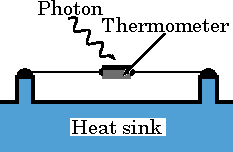
\includegraphics[width = 0.5\textwidth]{figures/simple_bolometer}
\caption[Schematic of a simple bolometer]{Schematic of a simple bolometer. An electrical thermometer is suspended above a heat sink by its wiring, which acts as a weak thermal link to the heat sink. One side of the thermometer is painted black to increase the absorption of incidental radiation. Incident power on the painted surface of the thermometer causes an increase in temperature, which can be measured. Heat is removed from the thermometer via its wiring.}
\label{fig:simpleBolometer}
\end{center}
\end{figure}
\par 
Figure~\ref{fig:simpleBolometer} illustrates a basic form of bolometer. A simple electrical thermometer (such as a piece of germanium) is suspended from a heat sink via its wiring. When power is absorbed, the temperature of the material increases accordingly, which results in a change in the material's electrical resistance. Heat is removed to the heat sink via the thermometer's wiring. This leads to one common issue experienced when designing a bolometric detector: it is highly desirable \reminder{hunt a reference for this} for the time constant of the detector (the minimum time between measurable detection events) to be as small as possible; this requires the absorbed power to be removed from the absorbing element as rapidly as possible, which in turn necessitates a strong thermal link between the absorber and the heat sink. However, increasing the thermal link between the heat sink and the absorber also has the effect of decreasing the sensitivity since the change in temperature within the absorber, for a given amount of absorber power, is also reduced. In most, cases one has to find a trade-off between speed of operation and the sensitivity of the detector. \reminder{Ref.}

\section{The History of Cold-Electron Bolometer Development}\label{sec:history}
Development of cold-electron bolometers has combined the developments of two fields to produce small, sensitive and fast bolometers. These fields are those of Hot-Electron Bolometers (HEBs) and tunnel-barrier superconducting electron refrigerators (also refereed to as microrefrigerators or e-fridges).
\par 
Although the phenomenon of heat transport between two superconductors separated by an insulator (\glstext{acr:SIS}) was first described by \textcite{Parmenter1961} as a way of improving superconductivity in one of the superconductors, it was not until \citeyear{Nahum1994} that heat extraction from electrons in a normal metal island (copper in this case) to a superconductor via an insulator (\glstext{acr:NIS}) was first observed by \textcite{Nahum1994}. From this point, several improvements were made, notably including the work of \textcite{Levio1996} who used a symmetric structure in which the normal island is sandwiched between the insulator-superconductor contacts (\glstext{acr:SINIS}); this allowed for replacement of the extracted electrons by carriers of lower energy, improving the cooling power of such a device, while also allowing for operation in both polarities. This approach of symmetric junctions allowed for electrons to be cooled from the lattice temperature of $300~\mathrm{mK}$ to close to $100~\mathrm{mK}$. An interesting development in this field, although not directly applicable to cold electron bolometers, was the work of \textcite{Clark2005}, who used \gls{acr:NIS} -based electron coolers to cool a membrane, as well as its contents, from $320~\mathrm{mK}$ to $225~\mathrm{mK}$; this work was also reported in Nature by \textcite{Pekola2005}.
\par 
Although first proposed in \citeyear{Parmenter1961} by \citeauthor{Parmenter1961}, enhancement of superconductivity through the use of \gls{acr:SIS} junction was first observed by \textcite{Chi1979}. However, \textcite{Manninen1999}, who used a slightly different arrangement whereby the a central superconductor is sandwiched by insulating contacts to a different superconductor (\glstext{acr:SIS2IS}), were the first to show directly that, in this arrangement, the electrons were being cooled below the temperature of the lattice.
\par 
The increasing interest in the these electron refrigerators led to the work of \textcite{Savin2001}, who first demonstrated that an effective electron refrigerator could be formed by replacing the normal metal island in a \glstext{acr:SINIS} with a highly-doped semiconductor (\glstext{acr:SSmS}). One immediate advantage of such a device was that, since it used naturally forming Schottky barriers in place of the oxide layers used in other types of device, fabrication was made simpler. \citeauthor{Savin2001} showed that such a device was capable of cooling the electrons in the semiconductor from the lattice temperature of $160~\mathrm{mK}$ to $120~\mathrm{mK}$. While this initial cooling was minimal, by \citeyear{Savin2003} \citeauthor{Savin2003} had improved these devices such that they were now capable of cooling from $150~\mathrm{mK}$ to less that $75~\mathrm{mK}$. Further improvements to \glstext{acr:SSmS} coolers were made by \cite{Prest2011} who---by using a strained, highly doped semiconductor as the central island---were able to cool the electrons in the semiconductor from $300~\mathrm{mK}$ to $174~\mathrm{mK}$.
\par 
While the use of the so-called \textit{hot-electron effect} to create a mixing heterodyne type detector was first described by \textcite{Arams1996}, the hot-electron bolometer was first envisaged by \textcite{Nahum1993}, who described a detector where incoming optical power heated the electrons in a normal metal absorber above the temperature of the lattice. The thermal isolation required to enable this independent heating of electrons comes from the fact that at low temperatures (typically less than $1~\mathrm{K}$), the inelastic collisions between the electrons and the atomic lattice are extremely infrequent, this is also factor in the effectiveness of the electron refrigerators described above. \citefirstauthor{Nahum1993} proposed the use of an insulating tunnel contact to a superconducting electrode to measure the temperature of the charges in the absorber. This is the same arrangement of a \glsfirst{acr:NIS} structure, as used in the electron refrigerators described above. They noted that, since the tunnelling current in a \gls{acr:NIS} junction is exponentially dependant on the temperature of the charges (as will be shown in Section~\ref{sec:theory-current} of Chapter~\ref{cha:theory}), this arrangement acts as an extremely sensitive thermometer.
\par 
There have been many notable publications and developments in the field of hot-electron bolometers. Of particular note is the work of \citeauthor{Karasik2011} which has shown that devices similar to those described by \citeauthor{Nahum1993} but using a thin strip of superconductor as the absorber, are capable of operating with a noise-equivalent power of $3 \times 10^{\nicefrac{-1}{2}}$ \parencite{Karasik2007,Karasik2011}. These levels of sensitivity make hot-electron bolometers an extremely exciting prospect for the next generation of both space and ground based telescopes. However, the speed of these devices is limited by the electron-phonon relaxation time \parencite[][reports a time constant of $30~\mathrm{\upmu s}$]{Karasik2007}. Furthermore, in order to achieve the thermal isolation required for highly sensitive detectors, these devices require the fabrication of absorbing islands with dimensions on the order of $1 \times 1~\mathrm{\upmu m}$ or smaller, with the need for contacts much smaller than this to be fabricated \parencite{Karasik2011}. The final undesirable feature of hot-electron bolometers is the need to degrade (slow) the thermal time constant to achieve high sensitivities \parencite{Karasik2000}. In order to increase the speed of the device, electrothermal feedback \parencite[as described by][]{Irwin1995} can be used. While this use of electrothermal feedback allowed microsecond scale thermal constants to be achieved, it also increased the complexity of the detector operation and restricted the biasing signal to a voltage bias. 
\par 
One important difference between the work of \citeauthor{Nahum1993} and \citeauthor{Karasik2000} is how their respective detectors were read out. As mentioned above, \citeauthor{Nahum1993} used a \gls{acr:NIS} tunnelling contact to act as an extremely sensitive electron thermometer. \citeauthor{Karasik2000} on the other hand, simply used the change in the resistance of the superconducting absorber (which was biased such that it was held on the superconducting transition) as the means of measuring the absorbed power (this is the same technique as used for the \glsfirst{acr:TES}).
\par 
The concept of using the \textit{cold-electron effect} that had been shown with electron refrigerator devices, combined with the thermal isolation of the electrons from the phonons used in hot-electron bolometers, was first proposed in \citeyear{Kuzmin1998} by \citeauthor{Kuzmin1998} who further elaborated on his idea in \citeyear{Kuzmin2000} and \citeyear{Kuzmin2003}. They described how using \glstext{acr:NIS} junctions could be used to lower the temperature of the electrons in a normal metal absorber to a rest temperature. Incident power absorbed within the absorber causes the electrons to heat up above the established rest temperature (much as in the case of the hot-electron bolometer). \citeauthor{Kuzmin1998} explained that the same \glstext{acr:NIS} junctions used to cool the electrons could be used as highly sensitive electron thermometers \parencite[as had been used by][]{Nahum1993}. Finally, \citeauthor{Kuzmin1998} showed that the time constant of such a detector would be limited by the electron tunnelling time as opposed to the thermal conductance between the electron and phonon systems. This integrated solution for both cooling and readout formed the first example of what could be called a cold-electron bolometer.\footnote{For this definition of a \glstext{acr:CEB}, the selection criterion was that the detector must be consciously designed to utilise direct electron cooling, with absorbed power heating the electrons above their cooled temperature.}
\par 
Since the original description of a cold-electron bolometer, there have been numerous publications on the topic. The most prolific author on the subject has been Leonid Kuzmin, who has shown the potential of such detectors to reach speeds in the order of nanoseconds \parencite{Kuzmin2004} and has been involved in the first optical measurement of the sensitivity of a metallic \glstext{acr:CEB} detector \parencite{Otto2013}, which was shown to have an amplifier-limited noise-equivalent power of $3.5 \times 10^{-17}~\mathrm{W\,Hz}^{\nicefrac{-1}{2}}$.
\par 
The work of Kuzmin et al. concentrated on cold-electron bolometers where the absorbing element was made from either a normal metal or a superconductor. As such, these devices are analogous to the \gls{acr:NIS} and \glstext{acr:SIS2} types of electron refrigerator described earlier in this section. Due to the success of \textcite{Prest2011} in achieving excellent levels of electron cooling, a logical step in the development of cold-electron bolometers was to replace the normal metal or superconducting absorber with a highly-degenerately-doped semiconductor. Such a device was first described and characterised by \textcite{Brien2014} and is further described in this thesis.

\section{The Advantages \& Disadvantages of Cold Electron Bolometers} \sectionmark{The Advantages \& Disadvantages of CEB\lowercase{s}}
\label{sec:advantages} 
Cold-elecron bolometers have been shown to have several advantages over other forms of bolometric detectors. Amongst these are: an extremely small thermal time constant \parencite[][shows that there is the potential for this to be as low as $10~\mathrm{ns}$]{Kuzmin2004}; high optical sensitivities \parencite[][achieved a noise-equivalent power of $3.5 \times 10^{-17}~\mathrm{W\,Hz}^{\nicefrac{-1}{2}}$---although this was limited by the readout amplifier]{Otto2013}; robust construction, since no suspended membrane or back etching is required to produce thermal isolation; and \parencite[as shown by][]{Salatino2014} a low susceptibility to cosmic rays.
\par 
One key disadvantage of cold-electron bolometers is that they cannot be connected together into an array in a way that facilitates a simple readout of the array. This is the case for all bolometric detectors since there is no trivial way of reading the resistance of a number of elements on a single readout line. While being a broad issue in the field of bolometric detectors, several schemes have been proposed and utilised to allow large arrays of bolometeric detectors---up to ten thousand pixels in the case of the SCUBA-2 instrument on the James Clark Maxwell Telescope \textcite{Holland2013}. The two most common schemes adopted are: \glsfirst{acr:FDM} and \glsfirst{acr:TDM}, whereby the signals from the various detectors are combined such that the signal from any individual detector only contributes a small part of the total signal received at the readout electronics. Time-division multiplexing operates by the signal switching sequentially between the sources in time intervals. For example, if ten devices are to be read in one second then every $100~ms$, the readout system would switch to measuring the next device; this requires that each detector has an amplifier or other component which can be switched on and off. Frequency-division multiplexing, on the other hand, works by modulating a carrier wave, which has a specific frequency. This modulation is typically in the carrier's frequency (i.e. shifting the frequency of the signal from the carrier's rest frequency), although parameters such as the carrier's amplitude or phase may also be used. As the value of the measured quantity varies, so too does the level of modulation. The frequency of the carrier wave associated with each device is different and is distributed across a frequency range. All the carrier waves in the frequency range are summed together allowing the information from several devices to be read on a single line. At a following stage in the readout system, these signals are demultiplexed by mixing the signal with a signal from a local oscillator whose frequency is the same as the original carrier. Using this approach, multiple signals are read simultaneously using a single line.
\par 
Multiplexing techniques have been used to allow larger arrays of bolometric detectors to be deployed. Some major (historical, current, or planned) instruments of particular note which have used these techniques include: the Keck array of telescopes measuring the polarisation of the cosmic microwave background (CMB) at the South Pole---each telescope uses time-division multiplexing to readout $512$ transition-edge sensors across 16 channels \parencite{Orlando2010}; SCUBA-2, a UK lead instrument at the John Clark Maxwell Telescope (JCMT) in Hawaii, which also utilises time-division multiplexing to readout an array of $10,240$ transition-edge sensors  across only eight channels \parencite{Holland2013}; the XMS instrument on NASA and ESA's jointly proposed \textit{IXO} mission plans to use frequency-division multiplexing to read $1,600$ pixels across $40$ channels \parencite{denHartog2011}; finally the SAFARI instrument on JAXA and ESA's joint \textit{SPICA} mission will use frequency-division multiplexing to readout arrays of $6,000$ detectors using $160$ channels.\footnote{In 2013 it was decided that the current scheme for delivering \textit{SPICA} would not produce `a robust and timely implementation' and \gls{acr:ESA} ceased to fund the development as of Autumn 2013 \parencite{ESA2014}. However, work is continuing \parencite{SRON2014} with the hope of launching \textit{SPICA} in 2025.}
\par 
Of particular interest to the field of cold-electron bolometers is the work of \textcite{Schmidt2005} who has proposed a scheme where frequency-division multiplexing is used to readout arrays of up to $10,000$ hot-electron bolometers. While the scheme devised by \citeauthor{Schmidt2005} was intended for use with hot-electron bolometers, due to the similarities between the two detector types, it should prove compatible with cold-electron bolometers, as well.
%
\section{Thesis Summary}
The preceding chapter has introduced the aim of this work. This is to introduce a new type of detector, the silicon cold-electron bolometer, and to characterise the performance and potential of such a detector. Two potential applications (astronomy and security) have been identified and briefly discussed. The general concepts relating to bolometeric detectors and the current status of cold-electron bolometers has been presented and the advantages and disadvantages of such detectors have also been discussed. 
\par 
Chapter~\chapterref{cha:theory} presents the theory of cold-electron bolometers. Key concepts are introduced, such as: tunnelling barriers and their fabrication, and detector response and sensitivity. In addition to this, the tunnelling current of a cold-electron bolometer is derived and, from this, it is shown that such a device is capable of direct electron cooling, the power associated with this electron cooling is then derived. The various sources of electrical noise present in such a system is discussed. This leads to the derivation of the ultimate sensitivity, the \glsfirst{acr:NEP}, of such a detector.
\par 
Chapter~\chapterref{cha:material} discusses the key properties of the two silicon materials used to fabricate the detectors studied in this thesis. This starts from a brief introduction to the energy structure of a semiconductor and continues to describe how this can be altered by the introduction of dopants. The mobility of charge carriers is discussed as are the key governing parameters of this mobility. Finally, the concept of strained semiconductors is introduced and an explanation as to how this can be utilised to improve the performance of a cold-electron bolometer is presented.
\par 
Chapter~\chapterref{cha:Design} describes the design and fabrication processes followed to produce the detectors studied in this thesis. The system used to couple radiation to the detector (a twin-slot antenna) is introduced. The general fabrication process flow used to manufacture to detectors is described, as are the defining parameters of the materials used to create the absorbers of these detectors.
\par 
Chapter~\chapterref{cha:testbeds} describes the cryogenic systems used to reach the low temperatures required by these detectors. A general description of each system is given and the basic working principles of the refrigeration system used within these cryostats is covered. The applications to which each system was best suited are also described. Finally, the design and manufacture of a device holder, incorporating a silicon lens, are described.
\par 
Chapter~\chapterref{cha:readout} describes the process of creating a readout and bias system for these detectors. Several iterations are described and each one is characterised to determine its suitability for the measurements in hand. In addition to these a novel concept of cross correlating the outputs of two matched amplifiers, operating in parallel, to reduce the effect of amplifier noise in a measurement, is presented. Both experimental data and a model are presented.
\par 
Chapter~\chapterref{cha:darkResults} presents results from the dark characterisation of these detectors. The current-voltage relationship is studied and from this the electron cooling is computed. This is performed for a detector with a unstrained-silicon absorber and a detector with a strained-silicon absorber. The mathematical stages needed to analyse the collected data are discussed.
\par 
Chapter~\chapterref{cha:opticalResults} describes the results found when the work described in Chapter~\chapterref{cha:darkResults} was repeated in the presence of incidental optical power. From this the responsivity of the detectors is found. The sensitivity of the detectors is found by measuring the noise generated within the detectors. In addition to this, the spectral response of the detectors is examined using a \glsfirst{acr:FTS}. Descrepancies from the expected form of this response are discussed and the initial modelling work of the antennae is revisited. Finally, a brief spectral study of the optical transmission of doped and strained silicon samples at terahertz frequencies is presented; from this, any limits to the usefulness of this material in these applications are discussed.
\par 
Chapter~\chapterref{cha:conclusion} concludes the thesis by summarising the key results found throughout this work and commenting on the overall performance of the detectors tested. Brief suggestions for further work in this field are presented.






